\chapter{Lec 05 - Decision Trees I}

\section{Decision Trees}
Decision trees (DTs) allow to learn \textbf{discrete} functions that are representable by a tree. Given a training set instance like the following one:
\begin{center}
    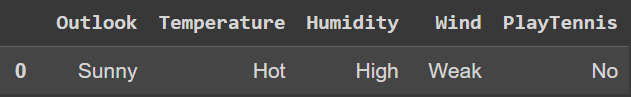
\includegraphics[scale=0.7]{images/Dataset instance.png}
\end{center}
\textbf{Attributes} are [$Outlook, Temperature, Humidity, Wind$], while $PlayTennis$ is the feature to predict (we want to predict if a day is suitable to play tennis). The values that $PlayTennis$ can take are called \textbf{classes}.
In a decision Tree:
\begin{itemize}
    \item An \textbf{inner node} corresponds to an attribute of an instance.
    \item A \textbf{branch} descending from a node corresponds to one of the possible values the attribute can assume.
    \item A \textbf{Leaf node} assigns a classification.
\end{itemize}
The classification of an instance works in the following way:
\begin{itemize}
    \item Start from the root
    \item Select the attribute attached to the current node
    \item Select a subtree following the branch corresponding to the value of that attribute in the instance.
    \item If we reach a leaf node we classify the instance with the associated label, else return to step 2.
\end{itemize}
Let's consider the following Decision Tree related to the \textit{tennis dataset} mentioned before.
\begin{center}
    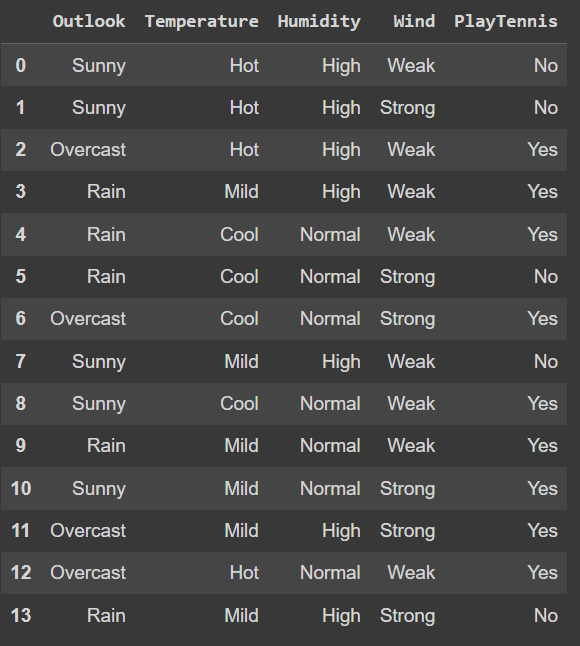
\includegraphics[scale=0.5]{images/layTennisDataset.png}
    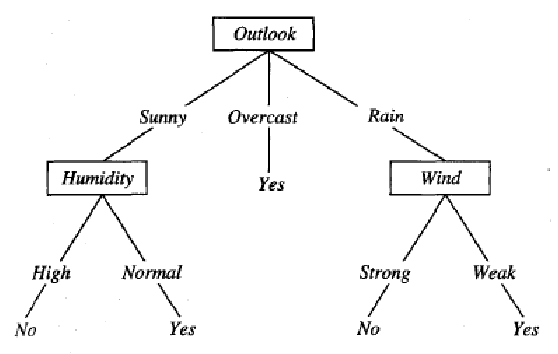
\includegraphics[scale=0.45]{images/decision tree playtennis.png}
\end{center}
The instance [O=Sunny, T=Hot, H=High, W=Strong] is classified with label \textit{NO} (not suitable to play tennis). In fact, following the path $O=Sunny \rightarrow H=High$ we end up in a leaf node with label 'NO'. Note that a decision tree can be represented as a boolean function:
\begin{itemize}
    \item Each path from the root to a leaf node codifies a conjunction of constraints on the attribute values of the instance.
    \item Different paths that lead to a same classification codify disjunctions of conjunctions.
\end{itemize}
So the classification can be seen as a series of \textbf{DNF} (disjunctive normal form) formulas, one DNF for each class. For example, DNF corresponding to \textit{YES} is (O=Sunny \textbf{and} H=Normal) \textbf{or} (O=Overcast) \textbf{or} (O=Rain \textbf{and} W=Week). This last feature, absent in most of the machine learning techniques, makes decision trees comprehensible and interpretable by humans. So they are particularly interesting for medical, biological and financial applications where interpreting a model is very important.
\subsection{DTs learning algorithm}
A recursive implementation of the \textbf{ID3} algorithm (the most popular learning algorithm for DTs) is the following:\newline
\textbf{ID3($S$, $A$)} Given a sample $S$ and a set of attributes $A$
\begin{itemize}
    \item If examples in $S$ are all of the same class $c$, return a leaf node with label $c$.
    \item if $A$ is empty, return a leaf node with label equals to the majority class\footnote{the class associated with the largest number of examples in $S$} in $S$.
    \item Select $a \in A$, the \textbf{optimal} attribute in $A$ and remove it from $A$ $(A = A - a)$.
    \item For each distinct value $v_{j}$ that $a$ can take in $S_{a}$, partition $S$ according to $v_{j}$ ($S_{a=v_{j}}$) and return the tree T having sub-trees the trees obtained by recursively calling \textbf{ID3}($S_{a=v_{j}}, A$).
\end{itemize}
Note that in the $4^{th}$ point of the algorithm, when you partition $S$ according to $v_{j}$, it is possible that in $S$ there are instances having only some of the possible values that the best attribute $a$ can take, so you have to consider only these values in that specific $S_{a}$ partition.

\subsection{Select optimal attribute}
Different learning algorithms for DTs mainly differ in how they select the optimal attributes. ID3 uses the concepts of \textbf{Entropy} and \textbf{Information Gain}.
\begin{itemize}
    \item \textbf{Entropy}: Let $C$ be the number of classes and $S_{c}$ the subset of $S$ of instances of class $c$, the entropy is computed as follows:
    \[E(S) = -\sum_{c=1}^{C}p_{c}log_{2}(p_{c})\]
    where $p_{c} = \frac{|S_{c}|}{|S|}$.
    In the case of binary classification (only two classes), it has the following shape:
    \begin{center}
        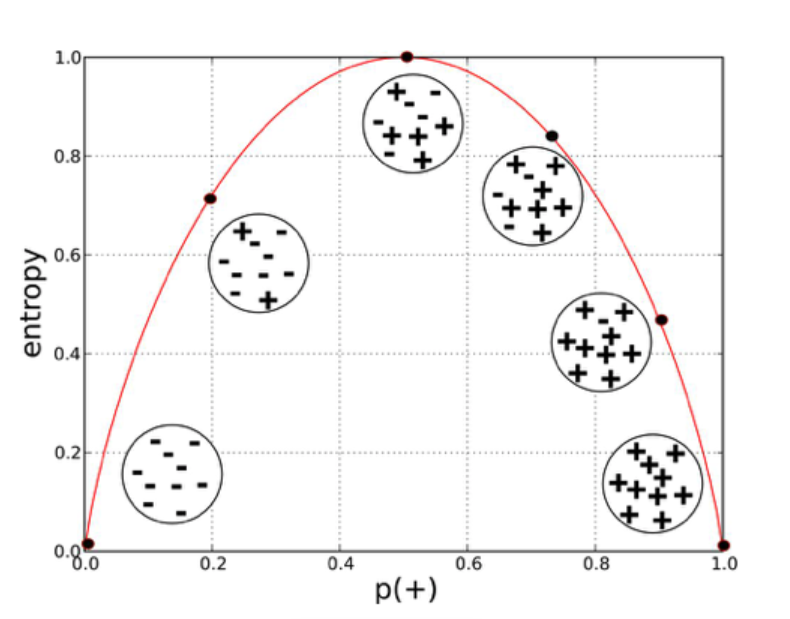
\includegraphics[scale=0.5]{images/entropy.png}
    \end{center}
    Entropy is lowest at the extremes, when $S$ either contains no positive instances or only positive instances (sample is pure without disorder) and it's highest where positive and negative instances are evenly split.
    
    \item \textbf{Information Gain:} The optimal attribute will be the one that maximizes the Information Gain $G(S,a)$
    \[G(S,a) = E(S) - \sum_{v \in V(a)}\frac{|S_{a=v}|}{|S|}E(S_{a=v})\]
    where 
    \begin{itemize}
        \item $S$ is the sample (could be the entire training set or a partition of it depending on which level of recursion we are in: see $4^{th}$ point of the ID3 algorithm.
        \item $a$ is the selected attribute.
        \item $E(S)$ is the total entropy of $S$.
        \item $V(a)$ is the set of distinct values that $a$ can take in $S_{a}$.
        \item $S_{a=v}$ is the partition of $S$ in which instances have the attribute $a$ equals to $v$.
    \end{itemize}
\end{itemize}
We can generalize the notion of Information Gain to other impurity measures:
\begin{itemize}
    \item \textbf{Cross-Entropy:} $I_{H} = -\sum_{c=1}^{C}p_{c}log_{2}(p_{c})$.
    \item \textbf{Gini Index:} $I_{G} = 1 - \sum_{c=1}^{C}(p_{c}^{2})$.
    \item \textbf{Misclassification:} $I_{E} = 1 - \max_{c}(p_{c})$.
\end{itemize}
Let $I$ be any of the impurity criteria mentioned above, the Information Gain definition becomes:
\[G(S,a) = I(S) - \sum_{v \in V(a)}\frac{|S_{a=v}|}{|S|}I(S_{a=v})\]
\subsection{DTs problems}
The information gain tends to favor attributes that can assume many possible values. \newline
\textbf{Example:} Consider a sample $S$ with an attribute consisting in dates. This attribute is likely going to be the one with maximum gain because each subset $S_{a=v}$, that is composed by \textbf{only one instance}, will be pure with zero impurity. In fact, the entropy of a subset with only one class is 0. \newline \newline
Another problem is the overfitting: The model is very accurate on training data but not on test data. 
\begin{center}
    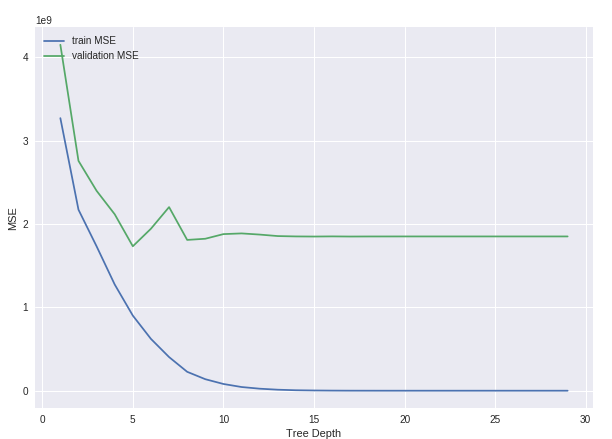
\includegraphics[scale=0.4]{images/overfitting dts.png}
\end{center}
We can observe that the problem increases as the number of nodes increases. A partial solution can be to set a minimal number of examples to accept on leaf nodes or limit the maximal depth of the tree (at a certain point i don't split $S$ anymore and i consider that node as a leaf with label the majority class in $S$).
\subsection{When to use DTs}
Decision trees are useful when dealing with problems having the following characteristics:
\begin{itemize}
    \item A fixed set of attributes and, for each attribute, a fixed set of values
    \item Discrete values for the attributes (decision trees can also be extended to deal with continuous values).
    \item Target function with discrete output values (classification problems).
    \item The target function can be approximated by disjunctions of boolean functions (Inductive bias).
    \item Training examples can contain noise (two or more instances with same attributes values but different classes) and missing values.
    
\end{itemize}
%You can find my implementation from scratch of ID3 algorithm on my GitHub(\url{https://github.com/riccardocappi/Machine_Learning_Course/blob/main/Decision_Trees_Python.ipynb}), Colab notebook(\url{https://colab.research.google.com/drive/1K2sytaFCfyT-FVMHNb7jvOi7bben_cah?usp=sharing}) or uploaded on the forum of ML course(\url{https://stem.elearning.unipd.it/mod/forum/discuss.php?d=2484}).
